%-----------------------------------------------------------------------------%
\chapter{\babEmpat}
\label{bab:4}
Metodologi yang telah dibahas sebelumnya diimplementasikan dengan bantuan program yang akan dijelaskan pada \bab{}~\ref{bab:4}. Secara garis besar, untuk mempersiapkan eksperimen dalam penelitian ini, terdapat tiga hal yang perlu dilakukan, yaitu persiapan data, pembangunan \pipeline{}, dan perancangan fitur yang divisualisasikan pada \gambar{}~\ref{fig:bagan}. Pada \subbab{}~\ref{subbab:4:Persiapan Data}, dijelaskan cara \parsing{} dan pembersihan data yang dilakukan untuk semua \file{} data. Kemudian, \subbab{}~\ref{subbab:4:Implementasi Model} membahas tentang implementasi sistem \ir{} dalam bentuk \pipeline{}. Setelah itu, proses ekstraksi fitur akan disampaikan pada \subbab{}~\ref{subbab:4:Ekstraksi Fitur}. Terakhir, pada \subbab{}~\ref{subbab:4:Evaluasi Model}, akan dijelaskan implementasi kode evaluasi dan perhitungan metrik hasil eksperimen.
\begin{figure}[!ht]
    \centering
    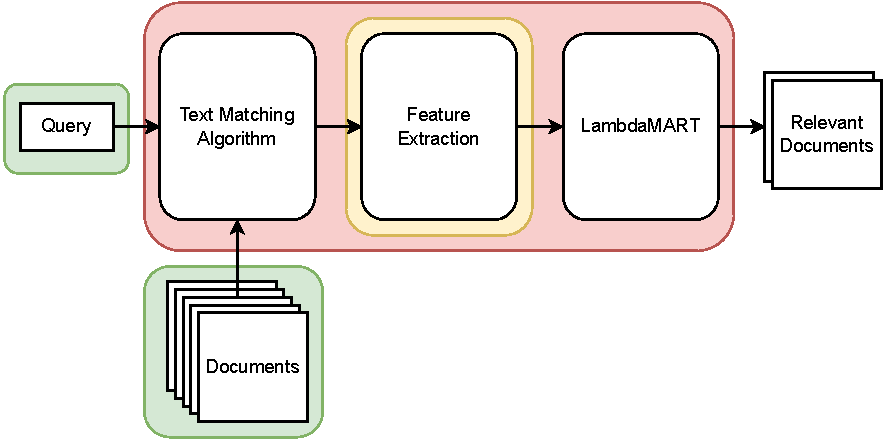
\includegraphics[scale=0.85]{assets/pdfs/GarisBesarImplementasi.pdf}
    \caption{Bagan implementasi yang perlu dilakukan. Pada bagian berwarna hijau, perlu dilakukan persiapan data kueri dan dokumen yang dilakukan dengan cara \parsing{} serta pembersihan karakter spesial, yang implementasinya dijelaskan pada \subbab{}~\ref{subbab:4:Persiapan Data}. Pada bagian berwarna merah, perlu dirancang suatu sistem \ir{} dengan arsitektur \cascaded{} yang diimplementasikan dengan membangun dan menyusun \pipeline{} serta membuat \textit{index} dengan bantuan \library{} pyterrier yang detailnya diberikan pada \subbab{}~\ref{subbab:4:Implementasi Model}. Kemudian, pada bagian oranye, perlu dilakukan berbagai ekstraksi fitur dari pasangan kueri-dokumen yang diperoleh dari \pipeline{} sebelumnya yang diimplementasikan pada \subbab{}~\ref{subbab:4:Ekstraksi Fitur}.}
    \label{fig:bagan}
\end{figure}
%-----------------------------------------------------------------------------%
%-----------------------------------------------------------------------------%
\section{Persiapan Data}
\label{subbab:4:Persiapan Data}
Pada tahap ini, peneliti melakukan persiapan data, meliputi \parsing{} dan pembersihan data. Pertama-tama, \parsing{} dilakukan untuk memberikan struktur pada data sehingga mudah untuk dianalisis maupun diproses lebih lanjut. Setelah itu, data yang telah di-\textit{parse} akan dibersihkan untuk memaksimalkan hasil dari sistem \ir{}. Pada \subbab{}~\ref{subbab:4:Data Pasal}, akan dijelaskan \parsing{} dan pembersihan data pasal (\corpus{}). Kemudian, \subbab{}~\ref{subbab:4:Data Pasangan Kasus-Dokumen Relevan} menyampaikan \parsing{} data kueri-pasal relevan secara lebih rinci.
%-----------------------------------------------------------------------------%
%-----------------------------------------------------------------------------%
\subsection{Data Pasal}
\label{subbab:4:Data Pasal}
Data pasal diberikan dalam bentuk \txt{} \file{} dan belum sepenuhnya terstruktur seperti yang ditunjukkan pada \gambar{}~\ref{gambar:TextFile}. Untuk itu, peneliti mengimplementasikan kode untuk melakukan pencocokan struktur dokumen legal pada setiap baris dari \file{} tersebut. Pencocokan struktur ini dilakukan untuk memilah bagian dari dokumen untuk dikonversi ke dalam bentuk tabel. Pada \kode{}~\ref{kode:parsing partition}, dapat dilihat bahwa dilakukan pencocokan baris terhadap struktur dokumen menggunakan \regex{} dengan bantuan \library{} re yang disediakan Python. Pencocokan tersebut dilakukan secara heuristik dengan memanfaatkan kata-kata kunci, seperti \textit{Part}, \textit{Chapter}, \textit{Section}, \textit{Subsection}, dan \textit{Article} yang diikuti penomoran dalam bentuk angka Arab atau Romawi, pada baris 3-13 dan 18-19. Selain itu, terdapat pencocokan struktur bagian yang mengandung satu atau lebih pasal pada baris 15-16. Kemudian, pada baris 21-22, terdapat pencocokan klausa berupa ayat atau kalimat hukum yang merupakan bagian terkecil dari hierarki struktur hukum dan sekaligus merupakan elemen dari suatu pasal atau \textit{article}. Fungsi memilah tersebut kemudian akan digunakan sebagai fungsi pembantu untuk melakukan \parsing{}.
\lstinputlisting[
language=python,
firstline=37,
lastline=58,
label={kode:parsing partition},
caption={Fungsi memilah struktur dokumen legal secara heuristik}
]{assets/codes/data_parsing.py}

Proses \parsing{} yang diimplementasikan pada \kode{}~\ref{kode:parsing pasal} merupakan algoritma sederhana yang mengiterasi setiap baris dalam \file{} kemudian melakukan salah satu dari dua hal, yaitu melakukan pencatatan pasal atau menyesuaikan struktur hierarki dari baris yang diiterasi. Pencatatan pasal diimplementasikan pada baris 9-11 yang melakukan penambahan klausa hukum untuk suatu pasal yang sedang diiterasi, serta pada baris 13-14 dan 35-36 yang melakukan finalisasi iterasi pasal dengan menambahkannya ke dalam \textit{list}. Selain itu, penyesuaian struktur hierarki hukum dapat dilihat pada baris 16-30 yang melakukan perubahan sesuai dengan struktur yang ditemui saat iterasi. Perubahan yang dimaksud terjadi ketika baris yang diiterasi beranjak dari suatu hierarki aturan ke hierarki lain yang sebanding atau lebih tinggi, sehingga data hierarki yang lebih rendah akan dihapus karena sudah tidak relevan dengan pasal pada bagian selanjutnya. Perhatikan bahwa walaupun masih dalam satu rantai pernyataan \lstinline{if-else}, baris 31-33 melakukan hal yang berbeda, yaitu mencatat baris yang menandakan awal mula iterasi pasal dan menyimpan kode unik yang dimiliki oleh setiap pasal.
\lstinputlisting[
language=python,
firstline=64,
lastline=101,
label={kode:parsing pasal},
caption={Fungsi \parsing{} pasal sebagai \corpus{}}
]{assets/codes/data_parsing.py}

Setelah itu, diimplementasikan fungsi penanganan karakter spesial pada \kode{}~\ref{kode:penanganan karakter spesial} untuk menghindari terjadinya \error{} pada saat proses \retrieval{} yang disebabkan oleh keberadaan karakter spesial.
\lstinputlisting[
language=python,
firstline=107,
lastline=109,
label={kode:penanganan karakter spesial},
caption={Penanganan karakter spesial}
]{assets/codes/data_parsing.py}

Kemudian, \kode{}~\ref{kode:tabelisasi} mengonversi \textit{list} yang didapat dari \kode{}~\ref{kode:parsing pasal} ke dalam bentuk tabel yang dapat dilihat pada baris 4-8. Perlu diperhatikan bahwa, pada baris 4, \parsing{} dilakukan dengan melewatkan baris pertama yang hanya berisi judul dari dokumen hukum. Kemudian, penghilangan karakter spesial dapat dilihat pada baris 10-11 dengan fungsi pembantu \kode{}~\ref{kode:penanganan karakter spesial}. Namun, seperti yang dijelaskan pada \subbab{}~\ref{subbab:3:Dataset} bahwa hilangnya keberadaan karakter-karakter spesial dapat menyebabkan makna semantik suatu kalimat untuk berubah karena bergantinya struktur kalimat tersebut. Oleh karena itu, diimplementasikan juga versi tanpa penghapusan karakter spesial yang dapat dilihat pada baris 16-18. Sehabis itu, kolom data tabel diatur ulang agar kolom yang esensial termasuk dalam kolom-kolom pertama sebelum dikembalikan.
\lstinputlisting[
language=python,
firstline=113,
lastline=132,
label={kode:tabelisasi},
caption={Konversi \corpus{} menjadi bentuk tabel}
]{assets/codes/data_parsing.py}

Sehabis implementasi fungsi \parsing{}, \kode{}~\ref{kode:tabelisasi} dijalankan dengan memasukkan lokasi \txt{} \file{} sebagai argumen dan hasilnya disimpan dalam variabel yang dapat ditemui pada \kode{}~\ref{kode:gunsi}. Terdapat 2 versi tabel yang disimpan, yaitu \lstinline{articles} sebagai tabel yang mengandung teks tanpa karakter spesial dan \lstinline{encoder_articles} yang masih mengandung karakter spesial pada teks.
\lstinputlisting[
language=python,
firstline=138,
lastline=139,
label={kode:gunsi},
caption={Melakukan \parsing{} \txt{} \file{} dan menyimpan hasil}
]{assets/codes/data_parsing.py}

Setelah menyimpan kedua tabel ke dalam variabel, dilakukan eksplorasi sederhana terhadap teks hasil \parsing{} untuk menyelidiki kemungkinan kesalahan dari implementasi \parsing{} yang telah dibuat. Berdasarkan eksplorasi tersebut, ditemukan bahwa ada beberapa duplikasi data sehingga dilakukan penghapusan data duplikat yang implementasinya dapat dilihat pada \kode{}~\ref{kode:pemusnahan duplikasi}.
\lstinputlisting[
language=python,
firstline=147,
lastline=148,
label={kode:pemusnahan duplikasi},
caption={Penanganan duplikasi data}
]{assets/codes/data_parsing.py}
Selain duplikasi data, ditemukan juga beberapa pasal valid namun tidak informatif yang tidak tereliminasi dengan \parsing{} secara heuristik yang telah diimplementasikan. Pasal tidak informatif tersebut merupakan pasal yang dihapus dari dokumen hukum seperti yang ditunjukkan pada \tabel{}~\ref{tabel:deleted article}.
\begin{table}[H]
    \centering
    \caption{Data hasil \parsing{} yang tidak berlaku dan sudah dihapus}
    \label{tabel:deleted article}
    \resizebox{\textwidth}{!}{%
        \begin{tabular}{lllp{0.125\linewidth}lp{0.225\linewidth}p{0.4\linewidth}}
        \toprule
        text & docno & part & chap & sect & subsect & subsubsect \\
        \midrule
        Article 208  Deleted & 208 & Real Rights & Ownership & Extent of Ownership & Content and Scope of Ownership & Scope of Ownership in Land \\
        Article 363  Deleted & 363 & Real Rights & Pledges & Pledges of Rights &  & Subject Matter of Pledges of Rights \\
        Article 365  Deleted & 365 & Real Rights & Pledges & Pledges of Rights &  & Requirements for Perfection of Pledges over Claims \\
        Article 367  Deleted & 367 & Real Rights & Pledges & Pledges of Rights &  & Collection of Claims by Pledgees \\
        Article 368  Deleted & 368 & Real Rights & Pledges & Pledges of Rights &  & Collection of Claims by Pledgees \\
        Article 480  Deleted & 480 & Claims & General Provisions & Extinction of Claims & Performance & Performance to Holder of Receipt \\
        Article 571  Deleted & 571 & Claims & Contracts & Sale & Effect of Sale & Buyer's Demand for Reimbursement of Expenses for Immovables Subject to Mortgage \\
        Article 635  Deleted & 635 & Claims & Contracts & Contracts for Work &  & Remuneration in Proportion to Benefit Received by Party Ordering Work \\
        \bottomrule
        \end{tabular}%
    }
\end{table}
Oleh karena itu, dilakukan pembersihan data dengan menggunakan pencocokan kata sederhana yang implementasinya terdapat pada \kode{}~\ref{kode:pemusnahan deleted}.
\lstinputlisting[
language=python,
firstline=184,
lastline=188,
label={kode:pemusnahan deleted},
caption={Pembersihan data}
]{assets/codes/data_parsing.py}
%-----------------------------------------------------------------------------%
%-----------------------------------------------------------------------------%
\subsection{Data Pasangan Kasus-Dokumen Relevan}
\label{subbab:4:Data Pasangan Kasus-Dokumen Relevan}
Pada tahapan selanjutnya, \parsing{} yang berbeda  dengan \subbab{}~\ref{subbab:4:Data Pasal} diimplementasikan untuk data pasangan kueri-pasal relevan yang telah diberikan pada \gambar{}~\ref{tabel:hasil parsing xml file}. Agar memudahkan proses \parsing{} suatu data XML, maka akan dimanfaatkan \library{} xml yang disediakan oleh Python yang memungkinkan akses elemen XML secara langsung. Pertama, diimplementasikan suatu fungsi pembantu untuk mengambil teks dari suatu elemen XML. Implementasi dari fungsi tersebut dapat ditemukan di \kode{}~\ref{kode:penculikan anak pertama}.
\lstinputlisting[
language=python,
firstline=204,
lastline=207,
label={kode:penculikan anak pertama},
caption={Fungsi pembantu untuk ekstraksi elemen XML}
]{assets/codes/data_parsing.py}

Kemudian, peneliti membuat implementasi \parsing{} untuk seluruh XML \file{} yang dapat dilihat pada \kode{}~\ref{kode:tabelisasi xml}. Perhatikan bahwa digunakan \library{} glob dari Python untuk memperoleh suatu daftar lokasi \file{} XML pada baris 6.
\lstinputlisting[
language=python,
firstline=209,
lastline=244,
label={kode:tabelisasi xml},
caption={Fungsi \parsing{} dan konversi ke dalam bentuk tabel}
]{assets/codes/data_parsing.py}
Dibandingkan dengan \parsing{} pada \subbab{}~\ref{subbab:4:Data Pasal}, \parsing{} untuk data XML lebih sederhana karena strukturnya yang sudah jelas. Dapat dilihat bahwa, fungsi tersebut diimplementasikan dengan mengiterasi setiap elemen \textit{pair} kemudian memasangkan kueri pada elemen \textit{t2} dengan setiap pasal relevan yang dapat ditemukan pada elemen \textit{t1}. Diimplementasikan juga untuk fungsi tanpa penghilangan karakter spesial pada baris ke-34.

Fungsi tersebut kemudian dijalankan dengan argumen lokasi \textit{directory} yang berisi data \training{} dan \testing{} sesuai dengan pembagian \dataset{} kompetisi \COLIEE{} 2023, untuk versi tanpa penghapusan karakter spesial, serta dengan penghapusan karakter spesial yang dapat dilihat pada \kode{}~\ref{kode:xunsi}. 
\lstinputlisting[
language=python,
firstline=250,
lastline=255,
label={kode:xunsi},
caption={Melakukan \parsing{} XML dan menyimpan hasil}
]{assets/codes/data_parsing.py}
%-----------------------------------------------------------------------------%
%-----------------------------------------------------------------------------%
\section{Implementasi Model}
\label{subbab:4:Implementasi Model}
Setelah data sudah siap dipakai, dipersiapkan implementasi program untuk membangun sistem \ir{} dalam bentuk \pipeline{}. \Pipeline{} yang dimaksud adalah suatu elemen pemrosesan data yang diatur secara berurutan dengan keluaran dari satu elemen akan menjadi masukan ke elemen berikutnya sampai diperoleh hasil akhir yang diinginkan. Dalam konteks \cascaded{} \ir{} yang ingin dirancang pada penelitian ini, akan dibentuk 3 buah \pipeline{}, yaitu \pipeline{} tahap \ranking{} pertama, \pipeline{} ekstraksi fitur, dan \pipeline{} tahap \ranking{} kedua menggunakan \lambdamart{}. Dalam penelitian ini, digunakan \library{} pyterrier dalam perancangan ketiga \pipeline{} tersebut. Agar dapat memanfaatkan pyterrier, perlu dieksekusi \kode{}~\ref{kode:init terrier} yang menjalankan program \lstinline{Terrier.jar} atau mengunduhnya terlebih dahulu sebelum dijalankan.
\begin{lstlisting}[language=Python, caption={Menjalankan program Terrier}, label={kode:init terrier}]
pt.init(version='5.x-SNAPSHOT', helper_version='0.0.8')
\end{lstlisting}

Sebelum melakukan proses \retrieval{}, agar dapat berjalan dengan efisien, dilakukan pembuatan indeks dokumen terlebih dahulu. Implementasi pembuatan indeks dapat dilihat pada \kode{}~\ref{kode:indexing}. Perhatikan bahwa, pada baris 1, dibentuk suatu objek yang dapat membuat indeks dalam bentuk \textit{blocks} dengan menerima parameter lokasi pembuatan indeks. Kemudian, pada baris 2, dibuat indeks untuk tabel pasal hasil \parsing{} \subbab{}~\ref{subbab:4:Persiapan Data}. Untuk membuat indeks tersebut, diberikan 2 argumen, pertama sebagai basis pembuatan \textit{inverted index} dan yang kedua adalah metadata yang ingin disimpan pada indeks.
\begin{lstlisting}[language=Python, caption={Pembentukan indeks}, label={kode:indexing}]
import pyterrier as pt

pd_indexer = pt.DFIndexer(os.path.join(DIR, 'coliee_index'), blocks=True)
index_ref = pd_indexer.index(articles["text"], articles)
\end{lstlisting}

Sehabis membentuk indeks, dilakukan perancangan \pipeline{} untuk analisis efektivitas berbagai \base{} \retriever{}. Pembentukan \pipeline{} tersebut diimplementasikan pada \kode{}~\ref{kode:init_retr}. Perhatikan bahwa pada baris 1-4 didaftarkan beberapa nama model atau algoritma \base{} \retrieval{}, kemudian untuk setiap model tersebut dibangun \pipeline{} \retrieval{} sebagai tahap \ranking{} pertama pada baris 6-8.
\begin{lstlisting}[language=Python, caption={Pembentukan \textit{Base retriever pipelines}}, label={kode:init_retr}]
models = ['BB2', 'BM25', 'CoordinateMatch', 'DFIC', 'DFIZ', 'DFR_BM25', 'DFRee',
          'DFReeKLIM', 'DirichletLM', 'Dl', 'DLH', 'DLH13', 'DPH', 'XSqrA_M',
          'Hiemstra_LM', 'IFB2', 'In_expB2', 'In_expC2', 'InB2', 'InL2',
          'Js_KLs', 'LemurTF_IDF', 'LGD', 'PL2', 'Tf', 'TF_IDF']

init_retrs = {model_name: pt.BatchRetrieve(index_ref, wmodel=model_name)
              for model_name
              in models}
\end{lstlisting}

Model yang terdaftar dalam bentuk \textit{dictionary} kemudian dipisahkan \textit{key} dan \textit{value}-nya menjadi 2 \textit{list}, yang berisi nama model dan \pipeline{}, untuk keperluan eksperimen \retrieval{}. Implementasi pemisahan tersebut dapat ditemukan di \kode{}~\ref{kode:init_retr_for_exp} yang melakukan iterasi terhadap setiap elemen pada \textit{dictionary}.
\begin{lstlisting}[language=Python, caption={Persiapan \textit{base retriever pipelines} untuk Eksperimen}, label={kode:init_retr_for_exp}]
model_names = []
base_pipelines = []

for name, init_retr in init_retrs.items():
    model_names.append(name)
    base_pipelines.append(init_retr)
\end{lstlisting}

Kedua \textit{list} yang didapat dari \kode{}~\ref{kode:init_retr_for_exp} digunakan sebagai argumen untuk eksperimen dengan memanfaatkan fungsi \lstinline{pyterrier.Experiment} yang implementasinya dapat dilihat pada \kode{}~\ref{kode:init_retr_exp}. Pada baris 7, diberikan argumen indeks dari \obm{} pada \textit{list} yang akan digunakan sebagai \baseline{} pada eksperimen ini. Selain itu, terdapat beberapa argumen lain pada baris 3-5, yang akan didefinisikan pada \subbab{}~\ref{subbab:4:Evaluasi Model}.
\begin{lstlisting}[language=Python, caption={Eksperimen berbagai model atau algoritma \base{} \retrieval{}}, label={kode:init_retr_exp}]
experiment_data = pt.Experiment(
    retr_systems=base_pipelines,
    topics=dev_topics,
    qrels=qrels,
    eval_metrics=metrics,
    names=model_names,
    baseline=model_names.index('BM25'))
\end{lstlisting}

Setelah melakukan seleksi model yang akan digunakan untuk analisis pada eksperimen-eksperimen berikutnya, akan dibangun \pipeline{} untuk \ranking{} pertama model-model tersebut. Implementasi pembentukan \pipeline{} dapat dilihat pada \kode{}~\ref{kode:pipe first}, serupa dengan pembentukan sebelumnya, dengan tambahan notasi \lstinline{% cut_off} untuk membatasi jumlah dokumen yang dikembalikan dalam tahap \ranking{} pertama pada sistem \cascaded{} \ir{}. Seperti yang telah dijelaskan pada \subbab{}~\ref{subbab:3:Definisi Tugas}, nilai dari \lstinline{cut_off} dalam sistem yang akan dibuat adalah 150.
\begin{lstlisting}[language=Python, caption={\Pipeline{} tahap \ranking{} pertama}, label={kode:pipe first}]
bm25 = pt.BatchRetrieve(index_ref, wmodel='BM25') % cut_off
tfidf = pt.BatchRetrieve(index_ref, wmodel='TF_IDF') % cut_off
dlh13 = pt.BatchRetrieve(index_ref, wmodel='DLH13') % cut_off
inl2 = pt.BatchRetrieve(index_ref, wmodel='InL2') % cut_off
dfr_bm25 = pt.BatchRetrieve(index_ref, wmodel='DFR_BM25') % cut_off
\end{lstlisting}

Kemudian, untuk setiap sistem, akan ditambahkan \pipeline{} yang mengambil teks dokumen dari indeks untuk keperluan ekstraksi fitur. Hal tersebut dilakukan karena teks tidak secara otomatis dikembalikan bersama proses \retrieval{} pada \ranking{} tahap pertama. Pada \kode{}~\ref{kode:pipe get text}, terdapat implementasi pembuatan \pipeline{} pengambilan teks dengan fungsi \lstinline{pyterrier.text.get_text} dan penyambungan kedua \pipeline{} dengan notasi \lstinline{>>}.
\begin{lstlisting}[language=Python, caption={Pengambilan teks dokumen pada \pipeline{}}, label={kode:pipe get text}]
pipe_bm25 = bm25 >> pt.text.get_text(index_ref, "text")
pipe_tfidf = tfidf >> pt.text.get_text(index_ref, "text")
pipe_dlh13 = dlh13 >> pt.text.get_text(index_ref, "text")
pipe_inl2 = inl2 >> pt.text.get_text(index_ref, "text")
pipe_dfr_bm25 = dfr_bm25 >> pt.text.get_text(index_ref, "text")
\end{lstlisting}

Sehabis itu, dengan cara yang sama, \pipeline{} gabungan yang didapat pada \kode{}~\ref{kode:pipe get text} akan disambung dengan \pipeline{} berikutnya, yaitu \pipeline{} ekstraksi fitur. Implementasi tersebut dapat ditemukan pada \kode{}~\ref{kode:pipe get feature}. \Pipeline{} \lstinline{all_features} bertugas melakukan komputasi nilai-nilai fitur yang menjadi usulan yang telah dibahas pada \subbab{}~\ref{subbab:3:Usulan Fitur} untuk setiap pasangan kueri-dokumen hasil keluaran dari \pipeline{} sebelumnya dan implementasinya baru akan dijelaskan pada \subbab{}~\ref{subbab:4:Ekstraksi Fitur}.
\begin{lstlisting}[language=Python, caption={\Pipeline{} ekstraksi fitur}, label={kode:pipe get feature}]
pipe_bm25_all = pipe_bm25 >> all_features
pipe_dlh13_all = pipe_dlh13 >> all_features
pipe_inl2_all = pipe_inl2 >> all_features
pipe_tfidf_all = pipe_tfidf >> all_features
pipe_dfr_bm25_all = pipe_dfr_bm25 >> all_features
\end{lstlisting}

Sebelum membangun \pipeline{} tahap \ranking{} terakhir, dipersiapkan terlebih dahulu fungsi untuk membangun model \lambdamart{} yang diimplementasikan pada \kode{}~\ref{kode:fun mart}. Dimanfaatkan \textit{library} xgb yang disediakan oleh XGBoost untuk mengonstruksi \lambdamart{} dengan menyesuaikan parameter optimasi, yaitu \textit{objective}, sebagai NDCG. Terdapat juga beberapa penyesuaian parameter lain, mengikuti saran \textit{library} pyterrier yang secara umum dilakukan untuk mencegah overfitting, seperti \lstinline{learning_rate} dan \lstinline{min_child_weight} yang lebih kecil, serta \lstinline{gamma} yang lebih besar.
\begin{lstlisting}[language=Python, caption={Pembentukan model \lambdamart{}}, label={kode:fun mart}]
import xgboost as xgb

def get_new_lambdamart():
    return xgb.sklearn.XGBRanker(
        objective='rank:ndcg',
        learning_rate=0.1,
        gamma=1.0,
        min_child_weight=0.1,
        random_state=42)
\end{lstlisting}

Kemudian, pada \kode{}~\ref{kode:pipe rerank init} dilakukan pencocokan antar nama, \pipeline{}, dan \reranker{} \lambdamart{} yang diperoleh pada \kode{}~\ref{kode:fun mart}. Penamaan yang digunakan untuk sistem \ir{} dengan \reranker{} mengikuti format \lstinline{<base_retriever> (Re-ranker)}. Perhatikan bahwa \lambdamart{} hanya dikonstruksi sekali untuk melakukan eksperimen karena setiap pelatihan yang dilakukan akan mengubah seluruh bobot pada model \lambdamart{}, dalam arti lain, pelatihan yang dilakukan akan independen terhadap hasil pelatihan-pelatihan sebelumnya.
\begin{lstlisting}[language=Python, caption={Pencocokan \pipeline{} \reranker{}}, label={kode:pipe rerank init}]
rerankers_pipe = {'BM25 (Re-ranker)': pipe_bm25_all,
                  'DLH13 (Re-ranker)': pipe_dlh13_all,
                  'InL2 (Re-ranker)': pipe_inl2_all,
                  'TF_IDF (Re-ranker)': pipe_tfidf_all,
                  'DFR_BM25 (Re-ranker)': pipe_dfr_bm25_all}

rerankers = {'BM25 (Re-ranker)': get_new_lambdamart(),
             'DLH13 (Re-ranker)': get_new_lambdamart(),
             'InL2 (Re-ranker)': get_new_lambdamart(),
             'TF_IDF (Re-ranker)': get_new_lambdamart(),
             'DFR_BM25 (Re-ranker)': get_new_lambdamart()}
\end{lstlisting}

Setelah dicocokkan nama dengan \pipeline{} yang sesuai, akan dilakukan penyambungan \pipeline{} ekstraksi fitur yang diperoleh pada \kode{}~\ref{kode:pipe get feature} dengan \pipeline{} tahap \ranking{} kedua, yaitu \pipeline{} \reranker{}. Konstruksi \pipeline{} \reranker{} memanfaatkan fungsi \lstinline{pyterrier.ltr.apply_learned_model} yang mengintegrasikan \lambdamart{} sebagai \pipeline{}. \kode{}~\ref{kode:pipe rerank append} mengimplementasi keseluruhan proses pembuatan \pipeline{} \reranker{} dan penyambungannya ke \pipeline{} sebelumnya.
\begin{lstlisting}[language=Python, caption={Pembuatan dan penyambungan \pipeline{} \reranker{}}, label={kode:pipe rerank append}]
pipelines_with_reranker = {
    reranker_name: rerankers_pipe[reranker_name] >> pt.ltr.apply_learned_model(
        rerankers[reranker_name], form="ltr")
    for reranker_name in rerankers
}\end{lstlisting}
Dengan penambahan \reranker{} tersebut, diharapkan dapat meningkatkan efektivitas proses \retrieval{} seperti salah satu contoh kasus yang dapat ditemui pada \tabel{}~\ref{tabel:hasil re-ranking}.

\begin{table}[H]
    \centering
    \caption{Cuplikan peningkatan hasil \reranking{}}
    \label{tabel:hasil re-ranking}
    \resizebox{\textwidth}{!}{%
        \begin{tabular}{llrrp{0.3\linewidth}p{0.3\linewidth}}
        \toprule
        qid & docno & rank\_before & rank\_after & query & text\\
        \midrule
        H18-25-E & 109 & 0 & 0 & a person who has manifested to a third party that he ... been granted authority of agency. & Article 109   1  A person who indicates to a third party ... other person has authority to represent in that act.\\
        H18-25-E & 107 & 4 & 3 & a person who has manifested to a third party that he ... been granted authority of agency. & Article 107  If an agent performs an act that falls within ... a person without authority to represent.\\
        H18-25-E & 110 & 16 & 11 & a person who has manifested to a third party that he ... been granted authority of agency. & Article 110  The provisions of the main clause of paragraph  1  of the ... agent has the authority as an agent.\\
        \bottomrule
    \end{tabular}%
    }
\end{table}

Sampai tahap ini, sistem \ir{} yang akan dianalisis sudah berhasil dikonstruksi. Oleh karena itu, berikutnya akan dilakukan persiapan untuk eksperimen. Pertama, dilakukan pendaftaran \base{} \retriever{} yang akan digunakan untuk pembanding saat eksperimen beserta pendekatan yang diusulkan dalam rupa sistem \ir{} yang implementasinya dapat ditemukan pada \kode{}~\ref{kode:daftar tanding}. Perlu diperhatikan bahwa, pada baris 13-14 dan 20-22, dilakukan pemisahan untuk sistem yang dilengkapi dengan \reranker{}. Hal tersebut dilakukan karena, dalam penelitian ini, dimanfaatkan suatu model \ml{}, sehingga terdapat kebutuhan pelatihan sebelum sistem dapat digunakan untuk menjalankan eksperimen.
\begin{lstlisting}[language=Python, caption={Pendaftaran model untuk eksperimen}, label={kode:daftar tanding}]
matching_alg = {
    'BM25': bm25,
    'TF_IDF': tfidf,
    'DLH13': dlh13,
    'InL2': inl2,
    'DFR_BM25': dfr_bm25
}

pipeline_agg = matching_alg | pipelines_with_reranker

pipeline_names = []
pipelines = []
pipeline_names_with_fit = []
pipelines_with_fit = []

for pipe_name, feature in pipeline_agg.items():
    pipeline_names.append(pipe_name)
    pipelines.append(feature)

    if pipe_name in pipelines_with_reranker:
        pipeline_names_with_fit.append(pipe_name)
        pipelines_with_fit.append(feature)
\end{lstlisting}

Pelatihan dilakukan untuk sistem yang memiliki \pipeline{} \reranker{} seperti yang telah dijelaskan sebelumnya. Untuk melatih \lambdamart{}, digunakan sebagian dari data \training{}, terlepas dari data yang digunakan untuk eksperimen maupun data \testing{}. \kode{}~\ref{kode:training reranker} mengandung implementasi program yang digunakan untuk melatih \reranker{} pada sistem \ir{} tersebut. Dapat dilihat bahwa, untuk setiap \pipeline{}, pelatihan menggunakan fungsi fit dengan argumen \lstinline{_train_topics} dan \lstinline{_val_topics} yang merupakan himpunan kueri yang berasal dari data \training{}, serta \lstinline{qrels} yang merupakan himpunan pasangan kueri-dokumen relevan.
\begin{lstlisting}[language=Python, caption={Pelatihan model \reranker{}}, label={kode:training reranker}]
for i, pipeline in enumerate(pipelines_with_fit):
    pipeline.fit(_train_topics, qrels, _val_topics, qrels)
\end{lstlisting}

Sesudah melatih seluruh \reranker{}, dilakukan eksperimen yang menggunakan data \lstinline{_val_topics} untuk evaluasi kinerja setiap sistem. Serupa dengan eksperimen sebelumnya, akan dimanfaatkan fungsi \lstinline{pt.Experiment} untuk penilaian kinerja sistem yang dapat dilihat implementasinya pada \kode{}~\ref{kode:experiment reranker}. Terdapat sedikit perbedaan argumen eksperimen, yaitu \lstinline{perquery}, untuk melakukan evaluasi kinerja pada tiap kueri.
\begin{lstlisting}[language=Python, caption={Eksperimen \retrieval{}}, label={kode:experiment reranker}]
experiment_data = pt.Experiment(
    retr_systems=pipelines,
    topics=_val_topics,
    qrels=qrels,
    eval_metrics=metrics,
    names=pipeline_names,
    perquery=True,
    verbose=True)
\end{lstlisting}

Metrik yang dihasilkan untuk setiap kueri tersebut kemudian diagregasi dengan bantuan fungsi \kode{}~\ref{kode:agg metric}. Perhatikan bahwa agregasi kinerja dilakukan dengan rata-rata.
\begin{lstlisting}[language=Python, caption={Agregasi metrik hasil eksperimen}, label={kode:agg metric}]
def agg_metrics(
    data: pd.DataFrame,
    drop_col: list[str] = ['qid'],
    group_col: Optional[str] = None,
) -> pd.DataFrame:
    _group_col = ['name']
    if group_col:
        _group_col.append(group_col)

    return data.drop(columns=drop_col).groupby(_group_col, as_index=False).mean()
\end{lstlisting}
%-----------------------------------------------------------------------------%
%-----------------------------------------------------------------------------%
\section{Ekstraksi Fitur}
\label{subbab:4:Ekstraksi Fitur}
Seperti yang telah disinggung di \subbab{}~\ref{subbab:4:Implementasi Model} bahwa terdapat \pipeline{} khusus yang akan digunakan untuk melakukan ekstraksi fitur, yaitu \pipeline{} \lstinline{all_features} pada \kode{}~\ref{kode:pipe get feature}. \subbab{}~\ref{subbab:4:Ekstraksi Fitur} membahas tentang implementasi proses ekstraksi fitur-fitur yang telah diusulkan pada \subbab{}~\ref{subbab:3:Usulan Fitur}. Secara garis besar, fitur yang akan diekstraksi dapat dibagi ke dalam 3 kelompok yang akan dijelaskan implementasinya pada \subbab{}~\ref{subbab:4:Ekstraksi Fitur:Atribut Kuantitatif Sederhana} untuk atribut kuantitatif sederhana, \subbab{}~\ref{subbab:4:Ekstraksi Fitur:Text Matching Score} untuk fitur skor \txt{} \matching{}, dan \subbab{}~\ref{subbab:4:Ekstraksi Fitur:Semantic Similarity} untuk pemanfaatan hasil \encoder{} sebagai fitur. Ketiga kelompok fitur tersebut akan diekstraksi dari hasil keluaran \pipeline{} sebelumnya, \kode{}~\ref{kode:pipe get text}, yang dapat dilihat cuplikannya pada \tabel{}~\ref{tabel:masukan feature extraction} yang mengandung hasil kembalian paling relevan dari \lstinline{pipe_bm25}. Dari hasil kembalian seperti yang telah dicontohkan, akan dimanfaatkan kolom \lstinline{query} yang merupakan teks kueri dan kolom \lstinline{text} yang merupakan teks dokumen untuk mendapatkan fitur sejumlah $40$. Proses ekstraksi tersebut divisualisasikan dalam bentuk diagram yang dilampirkan pada \gambar{}~\ref{Lampiran 1: Diagram Ekstraksi Fitur}.
\begin{table}[H]
    \centering
    \caption{Cuplikan hasil sebagai masukan \pipeline{} ekstraksi fitur}
    \label{tabel:masukan feature extraction}
    \resizebox{\textwidth}{!}{%
        \begin{tabular}{lrlrrp{0.225\linewidth}p{0.375\linewidth}}
        \toprule
        qid & docid & docno & rank & score & query & text \\
        \midrule
        H21-26-U & 654 & 620 & 0 & 18.152 & The cancellation of a partnership contract  shall solely become effective toward the future. & Article 620  If a lease is cancelled, the cancellation becomes effective solely toward the future. In such a case, the cancellation does not preclude a claim for compensation for loss or damage. \\
        \bottomrule
        \end{tabular}
    }
\end{table}

\subsection{Atribut Kuantitatif Sederhana}
\label{subbab:4:Ekstraksi Fitur:Atribut Kuantitatif Sederhana}
% \vspace{2mm}
% \noindent{}\textbf{Atribut Kuantitatif Sederhana}.

Berdasarkan yang telah dibahas pada \subbab{}~\ref{subbab:3:Usulan Fitur}, fitur usulan yang termasuk dalam kelompok ini hanya memanfaatkan atribut kuantitatif yang bisa didapatkan dari suatu teks, tanpa memperhitungkan kesamaan tekstual maupun semantik antara teks kueri dan teks dokumen. Terdapat 3 fitur usulan yang termasuk ke dalam kelompok ini, antara lain jumlah kata pada teks kueri, jumlah kata pada teks dokumen, dan selisih jumlah kata antara teks kueri dan teks dokumen. Pertama, diimplementasikan suatu fungsi untuk menghitung jumlah kata pada teks yang dapat dilihat pada \kode{}~\ref{kode:fungsi fitur jumlah kata}. Perhatikan bahwa nilai yang akan dimanfaatkan sebagai fitur, pada baris 7 dan 16, dikembalikan dalam bentuk \lstinline{numpy.ndarray}. Pembungkusan hasil perhitungan tersebut ke dalam \lstinline{numpy.ndarray} dilakukan agar dapat memanfaatkan fungsi penggabungan fitur yang disediakan pyterrier.


\begin{lstlisting}[language=Python, caption={Fungsi fitur jumlah kata}, label={kode:fungsi fitur jumlah kata}]
import numpy as np

def f_word_length(string: str) -> int:
    return len(string.split())

def word_length(string: str) -> np.ndarray[int]:
    return np.array([f_word_length(string)])

def f_word_length_diff(query: str, document: str) -> int:
    query_length = f_word_length(query)
    document_length = f_word_length(document)
    return abs(query_length - document_length)

def word_length_diff(query: str, document: str) -> np.ndarray[int]:
    diff = f_word_length_diff(query, document)
    return np.array([diff])
\end{lstlisting}

Fungsi yang telah didefinisikan pada \kode{}~\ref{kode:fungsi fitur jumlah kata} akan digunakan untuk mengekstraksi fitur dari pasangan kueri-dokumen yang dikembalikan oleh tahap \ranking{} pertama yang contohnya dapat dilihat pada \tabel{}~\ref{tabel:masukan feature extraction}. \Pipeline{} ekstraksi dibuat dengan fungsi \lstinline{pyterrier.apply.doc_features} menggunakan fungsi \lstinline{lambda} yang dapat ditemukan pada \kode{}~\ref{kode:fitur jumlah kata}. Pada baris 1-9, didapatkan fitur jumlah kata pada kueri maupun dokumen. Sementara itu, pada baris 11-14 diperoleh selisih antara jumlah kata yang terdapat pada kueri dan dokumen sebagai fitur.
\begin{lstlisting}[language=Python, caption={\Pipeline{} ekstraksi fitur jumlah kata}, label={kode:fitur jumlah kata}]
query_length = pt.apply.doc_features(
    lambda query_doc:
    word_length(query_doc['query'])
)

document_length = pt.apply.doc_features(
    lambda query_doc:
    word_length(query_doc['text'])
)

query_document_length_diff = pt.apply.doc_features(
    lambda query_doc:
    word_length_diff(query_doc['query'], query_doc['text'])
)
\end{lstlisting}








\subsection{Skor Berbasis \textit{Text Matching}}
\label{subbab:4:Ekstraksi Fitur:Text Matching Score}
% \vspace{2mm}
% \noindent{}\textbf{Text Matching Score}

Pada kelompok ini, akan dimanfaatkan model-model \base{} \retriever{} untuk melakukan perhitungan skor seperti kolom \textit{score} yang dapat ditemukan pada \tabel{}~\ref{tabel:masukan feature extraction}. Skor yang didapat dari perhitungan model tersebut kemudian akan digunakan sebagai salah satu fitur. Pada \kode{}~\ref{kode:pembentukan model untuk ekstraksi fitur} akan dibentuk \pipeline{} untuk setiap model \base{} \retriever{} yang akan digunakan sebagai fitur. Perlu diperhatikan bahwa dilakukan penghapusan 5 model \base{} \retriever{} yang terpilih untuk sistem \ir{}, namun hal tersebut hanya dilakukan agar tidak terjadi ekstraksi lebih dari satu kali untuk model yang sama.
\begin{lstlisting}[language=Python, caption={\Pipeline{} ekstraksi fitur skor \base{} \retriever{}}, label={kode:pembentukan model untuk ekstraksi fitur}]
base_models = ['BM25', 'TF_IDF', 'DLH13', 'InL2', 'DFR_BM25']
other_models = ['BB2', 'BM25', 'CoordinateMatch', 'DFIC', 'DFIZ', 'DFR_BM25', 'DFRee',
                'DFReeKLIM', 'DirichletLM', 'Dl', 'DLH', 'DLH13', 'DPH', 'XSqrA_M',
                'Hiemstra_LM', 'IFB2', 'In_expB2', 'In_expC2', 'InB2', 'InL2',
                'Js_KLs', 'LemurTF_IDF', 'LGD', 'PL2', 'Tf', 'TF_IDF']

for _model in base_models:
    other_models.remove(_model) 

other_matching_alg = [pt.BatchRetrieve(index_ref, wmodel=model_name) % cut_off
                      for model_name in other_models]
\end{lstlisting}

Selain perhitungan dari model-model berbasis \txt{} \matching{} tersebut, dalam kelompok ini juga terdapat fitur usulan \lstinline{jaccard} dan \lstinline{rake_jaccard} seperti yang telah dijelaskan pada \subbab{}~\ref{subbab:3:Usulan Fitur}. Sebelum membentuk \pipeline{} untuk kedua fitur tersebut, diimplementasikan algoritma RAKE terlebih dahulu. Perlu diperhatikan bahwa untuk mengimplementasi algoritma RAKE, akan digunakan beberapa \library{}, yaitu nltk dan rake\_nltk. Kemudian, agar algoritma dapat diimplementasikan juga untuk bahasa Indonesia, maka diperlukan beberapa data yang perlu diunduh terlebih dahulu. \kode{}~\ref{kode:dependency rake} melakukan pengunduhan data \textit{stopwords} dan \textit{punkt} sebagai dependensi dari \library{} rake\_nltk, serta pengunduhan \textit{stopwords} untuk bahasa Indonesia\footnote{https://github.com/stopwords-iso/stopwords-id.git}.
\begin{lstlisting}[language=Python, caption={Dependensi algoritma RAKE}, label={kode:dependency rake}]
import json
import nltk

from rake_nltk import Rake
from nltk.tokenize import RegexpTokenizer

assert nltk.download('stopwords')
assert nltk.download('punkt')

with open(IDN_STOPWORDS_DIR) as f:
  idn_stopwords = json.load(f)
\end{lstlisting}

Setelah dependensi berhasil diunduh, RAKE diimplementasikan dengan bantuan \textit{library} \lstinline{rake_nltk} yang dapat ditemukan pada \kode{}~\ref{kode:rake}. Ekstraksi dilakukan dengan menginisialisasi \lstinline{rake_nltk.Rake} menggunakan daftar \textit{stopwords}, sesuai bahasa yang diinginkan, sebagai argumen. Kemudian, kata kunci atau frasa penting dalam suatu teks dapat diekstraksi dengan memanggil fungsi seperti pada baris 10.
\begin{lstlisting}[language=Python, caption={Implementasi RAKE}, label={kode:rake}]
def extract_keywords_rake(
    text: str,
    language: Optional[str]=None,
    with_scores: bool=False
):
    if language is None or language == 'english':
        r = Rake()
    elif language == 'indonesian':
        r = Rake(stopwords=idn_stopwords)
    r.extract_keywords_from_text(text)
    
    return r.get_ranked_phrases()
\end{lstlisting}

Kesamaan jaccard diimplementasikan pada \kode{}~\ref{kode:fungsi fitur jaccard}, secara spesifik pada dua baris pertama. Fungsi tersebut menerima dua buah himpunan kata kemudian dilakukan pembagian jumlah irisan kata dari himpunan-himpunan tersebut oleh jumlah kata unik dari kedua himpunan. Kemudian, fungsi tersebut dimanfaatkan dengan beberapa kombinasi metode, antara lain dengan RAKE pada baris 14-19 atau \regex{} pada baris 22-24. 
Untuk metode \regex{}, kesamaan jaccard dihitung berdasarkan himpunan kata yang ditemukan dalam teks. Sementara itu, metode RAKE menghitung kesamaan jaccard berdasarkan himpunan frasa atau kata penting yang berhasil diekstraksi dari teks.
\begin{lstlisting}[language=Python, caption={Fungsi fitur jaccard}, label={kode:fungsi fitur jaccard}]
def f_jaccard(query_set, document_set):
  return len(query_set & document_set) / len(query_set | document_set)

VALID_LANGUAGE = [None, 'english', 'indonesian']
def jaccard(
    query: str,
    document: str,
    rake: bool=False,
    language: Optional[str]=None
):
  query = query.lower()
  document = document.lower()

  if rake:
    if language not in VALID_LANGUAGE:
        raise ValueError("language must be one of %r" % VALID_LANGUAGE)

    query_set = set(extract_keywords_rake(query, language=language))
    document_set = set(extract_keywords_rake(document, language=language))

  else:
    tokenizer = RegexpTokenizer(r'[\w]+')
    query_set = set(tokenizer.tokenize(query))
    document_set = set(tokenizer.tokenize(document))

  return np.array([
      f_jaccard(query_set, document_set)
  ])
\end{lstlisting}


Setelah diimplementasikan fungsi kesamaan jaccard, dibentuk dua buah \pipeline{}, versi dengan RAKE dan tanpa RAKE, yang dapat ditemukan pada \kode{}~\ref{kode:fitur jaccard}. Pada implementasi tersebut, versi \pipeline{} dengan \regex{} dapat ditemukan di baris 1-4, sedangkan versi \pipeline{} dengan RAKE dapat dilihat pada baris 6-9.
\begin{lstlisting}[language=Python, caption={\Pipeline{} ekstraksi fitur jaccard}, label={kode:fitur jaccard}]
jaccard_score = pt.apply.doc_features(
    lambda query_doc:
    jaccard(query_doc['query'], query_doc['text'], rake=False)
)

rake_jaccard_score = pt.apply.doc_features(
    lambda query_doc: jaccard(
        query_doc['query'], query_doc['text'], rake=True)
)
\end{lstlisting}


\subsection{Semantic Similarity}
\label{subbab:4:Ekstraksi Fitur:Semantic Similarity}
% \vspace{2mm}
% \noindent{}\textbf{Semantic Similarity}
Untuk mendapatkan makna semantik dari suatu teks, digunakan \encoder{} dari \llm{} (\LLM{}). Model tersebut menerima sebuah teks dan mengeluarkan vektor representasi dari teks tersebut yang dapat dikaitkan dengan makna semantik dari teks atau yang biasa dikenal sebagai vektor \embedding{}. Terdapat beberapa model LLM yang diusulkan untuk dimanfaatkan \encoder{}-nya, seperti \bert{}\footnote{https://huggingface.co/google-bert/bert-base-uncased} dan \tfive{}\footnote{https://huggingface.co/BeIR/query-gen-msmarco-t5-base-v1}. Kedua model \LLM{} tersebut diunduh dan dimuat konfigurasinya oleh \kode{}~\ref{kode:load llms}.
\begin{lstlisting}[language=Python, caption={\textit{Load} \encoder{} dan model yang sudah dilatih}, label={kode:load llms}]
from transformers import BertTokenizer, BertModel, \
    T5Tokenizer, T5EncoderModel, PreTrainedTokenizer, PreTrainedModel

bert_tokenizer = BertTokenizer.from_pretrained('google-bert/bert-base-uncased')
bert_model = BertModel.from_pretrained('google-bert/bert-base-uncased')

t5_tokenizer = T5Tokenizer.from_pretrained('BeIR/query-gen-msmarco-t5-base-v1')
t5_model = T5EncoderModel.from_pretrained('BeIR/query-gen-msmarco-t5-base-v1')
\end{lstlisting}


Setelah memuat model beserta \textit{tokenizer} untuk \bert{} dan \tfive{}, diimplementasikan fungsi pada \kode{}~\ref{kode:input encoder} untuk memperoleh vektor dari semua \hs{} yang kombinasinya akan diuji pada eksperimen selanjutnya. Perhatikan bahwa teks perlu di-\textit{tokenize} terlebih dahulu untuk mendapatkan representasinya dalam bentuk angka sebelum dapat dimasukkan ke \encoder{}. Proses \textit{tokenize} tersebut diimplementasikan pada baris ke-6 dengan argumen tambahan \lstinline{truncation} yang akan memotong jumlah \textit{token} yang dikembalikan jika sudah melebihi batas. Kemudian daftar \textit{token} yang dikembalikan akan menjadi masukan dari \encoder{}, begitu juga untuk argumen \lstinline{output_hidden_states} yang diatur untuk bernilai \lstinline{True} agar \encoder{} mengembalikan seluruh keluaran \hs{}.

\begin{lstlisting}[language=Python, caption={Fungsi mendapatkan keluaran dari \encoder{}}, label={kode:input encoder}]
def get_model_outputs(
    string: str,
    tokenizer: PreTrainedTokenizer,
    model: PreTrainedModel
):
    encoded_string = tokenizer(string, return_tensors='pt', truncation=True)
    model_output = model(**encoded_string, output_hidden_states=True)
    return model_output
\end{lstlisting}


Pada \kode{}~\ref{kode:get hss} berikut, diimplementasikan pengambilan keluaran beberapa \hs{s} dari \encoder{} yang dipakai. Bisa dilihat bahwa \lstinline{last_hidden_state_feature_vector} merupakan fungsi yang mengembalikan nilai keluaran dari \hs{} terakhir, sedangkan \lstinline{all_hidden_state_feature_vector}  mengembalikan nilai keluaran dari seluruh \hs{s}.
\begin{lstlisting}[language=Python, caption={Fungsi pengambilan \hs{}}, label={kode:get hss}]
def last_hidden_state_feature_vector(
    string: str,
    tokenizer: PreTrainedTokenizer,
    model: PreTrainedModel
):
    model_output = get_model_outputs(
        string=string, tokenizer=tokenizer, model=model)
    return model_output.last_hidden_state

def all_hidden_state_feature_vector(
    string: str,
    tokenizer: PreTrainedTokenizer,
    model: PreTrainedModel
):
    model_output = get_model_outputs(
        string=string, tokenizer=tokenizer, model=model)
    return model_output.hidden_states
\end{lstlisting}


Setelah diimplementasikan fungsi yang mengambil beberapa keluaran \hs{s}, pada \kode{}~\ref{kode:get cls}, diberikan implementasi pengambilan vektor pertama dari suatu \hs{}. Perhatikan bahwa digunakan \library{} torch untuk mengonversi keluaran model yang berupa \lstinline{tuple} menjadi bentuk \lstinline{torch.tensor}. Sehabis itu, dilakukan pengambilan vektor \textit{token} pertama dari setiap \hs{s} dengan pemotongan \lstinline{[:, 0, :]}. Perhatikan bahwa terdapat 3 dimensi dari hasil kembalian \lstinline{all_hidden_state_feature_vector} yang secara terurut mewakilkan \hs{}, \textit{token}, dan vektor.
\begin{lstlisting}[language=Python, caption={Pengambilan vektor pertama keluaran \hs{}}, label={kode:get cls}]
import torch

def get_cls(
    string: str,
    tokenizer: PreTrainedTokenizer,
    model: PreTrainedModel,
):
    model_output = all_hidden_state_feature_vector(
        string=string,
        tokenizer=tokenizer,
        model=model
    )
    hidden_states_tensor = torch.cat(model_output)
    return hidden_states_tensor[:, 0, :]
\end{lstlisting}





Kemudian, diimplementasikan beberapa metode pemanfaatan vektor dari keluaran \hs{s} yang akan dijadikan sebagai representasi teks, seperti yang telah dijelaskan pada \subbab{}~\ref{subbab:3:Usulan Fitur}. Implementasi pemanfaatan vektor tersebut dapat dilihat di \kode{}~\ref{kode:get which hs}. Perlu diperhatikan bahwa dilewatkan \hs{} pertama pada \lstinline{sum_ahs_cls} karena, untuk \bert{}, keluaran \hs{} yang dikembalikan sejumlah 13 dengan \hs{} pertama yang lebih dikenal sebagai \embedding{}.
\begin{lstlisting}[language=Python, caption={Metode pengambilan vektor dari \hs{}}, label={kode:get which hs}]
def lhs_mean(
    string: str,
    tokenizer: PreTrainedTokenizer,
    model: PreTrainedModel
):
    model_output = last_hidden_state_feature_vector(
        string=string,
        tokenizer=tokenizer,
        model=model
    )
    return model_output.mean(dim=1).flatten().detach()

def fhs_cls(
    string: str,
    tokenizer: PreTrainedTokenizer,
    model: PreTrainedModel,
):
    hidden_states_cls = get_cls(string=string, tokenizer=tokenizer, model=model)
    return hidden_states_cls[0].detach()

def lhs_cls(
    string: str,
    tokenizer: PreTrainedTokenizer,
    model: PreTrainedModel,
):
    hidden_states_cls = get_cls(string=string, tokenizer=tokenizer, model=model)
    return hidden_states_cls[-1].detach()

def stlhs_cls(
    string: str,
    tokenizer: PreTrainedTokenizer,
    model: PreTrainedModel,
):
    hidden_states_cls = get_cls(string=string, tokenizer=tokenizer, model=model)
    return hidden_states_cls[-2].detach()

def sum_ahs_cls(
    string: str,
    tokenizer: PreTrainedTokenizer,
    model: PreTrainedModel,
):
    hidden_states_cls = get_cls(string=string, tokenizer=tokenizer, model=model)
    return hidden_states_cls[1:].sum(dim=0).detach()

def sum_lfhs_cls(
    string: str,
    tokenizer: PreTrainedTokenizer,
    model: PreTrainedModel,
):
    hidden_states_cls = get_cls(string=string, tokenizer=tokenizer, model=model)
    return hidden_states_cls[-4:].sum(dim=0).detach()

def concat_lfhs_cls(
    string: str,
    tokenizer: PreTrainedTokenizer,
    model: PreTrainedModel,
):
    hidden_states_cls = get_cls(string=string, tokenizer=tokenizer, model=model)
    return hidden_states_cls[-4:].flatten().detach()
\end{lstlisting}








Sehabis mendefinisikan beberapa metode pengambilan vektor keluaran \hs{}, fungsi tersebut dibungkus dalam fungsi \lstinline{lambda} yang dapat ditemukan pada \kode{}~\ref{kode:fungsi lambda encoder} untuk beberapa usulan fitur yang akan diuji. Terdapat 7 metode pengambilan yang akan diuji untuk penggunaan \bert{}, diantaranya \lstinline{get_bert_lhs_mean} yang merupakan usulan dari peneliti, kemudian 6 sisanya merupakan usulan dari~\citet{devlin2018bert}. Selain menggunakan \bert{}, diuji juga 2 metode pemanfaatan vektor dengan menggunakan \encoder{} \tfive{} mengikuti usulan~\citet{ni2021sentence}.
\begin{lstlisting}[language=Python, caption={Fungsi lambda pengambilan vektor}, label={kode:fungsi lambda encoder}]
get_bert_lhs_mean = lambda st: lhs_mean(st, bert_tokenizer, bert_model)
get_bert_fhs_cls = lambda st: fhs_cls(st, bert_tokenizer, bert_model)
get_bert_lhs_cls = lambda st: lhs_cls(st, bert_tokenizer, bert_model)
get_bert_stlhs_cls = lambda st: stlhs_cls(st, bert_tokenizer, bert_model)
get_bert_sum_ahs_cls = lambda st: sum_ahs_cls(st, bert_tokenizer, bert_model)
get_bert_sum_lfhs_cls = lambda st: sum_lfhs_cls(st, bert_tokenizer, bert_model)
get_bert_concat_lfhs_cls = lambda st: concat_lfhs_cls(st, bert_tokenizer, bert_model)

get_t5_lhs_mean = lambda st: lhs_mean(st, t5_tokenizer, t5_model)
get_t5_lhs_cls = lambda st: lhs_cls(st, t5_tokenizer, t5_model)
\end{lstlisting}


Terdapat 9 fitur usulan yang memanfaatkan keluaran dari \encoder{}, secara spesifik keluaran yang telah didefinisikan \kode{}~\ref{kode:fungsi lambda encoder}. Pertama, digunakan fungsi \lstinline{lambda} yang telah didefinisikan untuk mendapatkan vektor representasi dari kueri dan dokumen. Kemudian, dilakukan komputasi kesamaan antara kedua vektor tersebut menggunakan \textit{cosine similarity} yang memanfaatkan \library{} torch, khususnya fungsi \lstinline{torch.nn.functional.cosine_similarity}. Implementasi perhitungan tersebut dapat ditemukan pada \kode{}~\ref{kode:cos}
\begin{lstlisting}[language=Python, caption={Fungsi ekstraksi fitur \textit{cosine\_similarity}}, label={kode:cos}]
def f_cosine_similarity(query_vec, document_vec):
    return torch.nn.functional.cosine_similarity(
        query_vec, document_vec, dim=0
    )

def enc_cos(query: str, document: str, get_vec: Callable):
    query_feature_vec = get_vec(query)
    docrel_feature_vec = get_vec(document)
    return np.array([f_cosine_similarity(query_feature_vec, docrel_feature_vec)])
\end{lstlisting}

Kemudian, untuk setiap usulan metode pengambilan vektor, dibangun \pipeline{} ekstraksi fitur yang dapat ditemukan pada \kode{}~\ref{kode:fitur cos}.
\begin{lstlisting}[language=Python, caption={\Pipeline{} ekstraksi fitur \textit{cosine\_similarity} dari \encoder{}}, label={kode:fitur cos}]
bert_lhs_mean = pt.apply.doc_features(lambda query_doc: enc_cos(
    query_doc['query'], query_doc['text'], get_bert_lhs_mean))
bert_fhs_cls = pt.apply.doc_features(lambda query_doc: enc_cos(
    query_doc['query'], query_doc['text'], get_bert_fhs_cls))
bert_lhs_cls = pt.apply.doc_features(lambda query_doc: enc_cos(
    query_doc['query'], query_doc['text'], get_bert_lhs_cls))
bert_stlhs_cls = pt.apply.doc_features(lambda query_doc: enc_cos(
    query_doc['query'], query_doc['text'], get_bert_stlhs_cls))
bert_sum_ahs_cls = pt.apply.doc_features(lambda query_doc: enc_cos(
    query_doc['query'], query_doc['text'], get_bert_sum_ahs_cls))
bert_sum_lfhs_cls = pt.apply.doc_features(lambda query_doc: enc_cos(
    query_doc['query'], query_doc['text'], get_bert_sum_lfhs_cls))
bert_concat_lfhs_cls = pt.apply.doc_features(lambda query_doc: enc_cos(
    query_doc['query'], query_doc['text'], get_bert_concat_lfhs_cls))

t5_lhs_mean = pt.apply.doc_features(lambda query_doc: enc_cos(
    query_doc['query'], query_doc['text'], get_t5_lhs_mean))
t5_lhs_cls = pt.apply.doc_features(lambda query_doc: enc_cos(
    query_doc['query'], query_doc['text'], get_t5_lhs_cls))
\end{lstlisting}


\subsection{\Pipeline{} Ekstraksi Fitur}
\label{subbab:4:Ekstraksi Fitur:Pipeline Ekstraksi Fitur}
\Pipeline{} ekstraksi fitur yang telah didefinisikan sebelumnya akan dikelompokkan menjadi satu \pipeline{} \lstinline{all_features}. Kelompok \pipeline{} dibentuk dengan menggunakan notasi \lstinline{**} yang implementasinya dapat dilihat pada \kode{}~\ref{kode:combine ekstraksi fitur}.

\begin{lstlisting}[language=Python, caption={Penggabungan \pipeline{} ekstraksi fitur}, label={kode:combine ekstraksi fitur}]
query_doc_features = query_length ** document_length ** query_document_length_diff
jaccard_scores = jaccard_score ** rake_jaccard_score
best_matching_alg_scores = dlh13 ** inl2 ** dfr_bm25
common_matching_alg_scores = bm25 ** tfidf
enc_cos_scores = bert_lhs_mean ** t5_lhs_mean ** bert_fhs_cls ** \
    bert_lhs_cls ** t5_lhs_cls ** bert_stlhs_cls ** \
    bert_sum_ahs_cls ** bert_sum_lfhs_cls ** bert_concat_lfhs_cls

other_matching_alg_scores = None
for alg in other_matching_alg:
    if other_matching_alg_scores is None:
        other_matching_alg_scores = alg
    else:
        other_matching_alg_scores = other_matching_alg_scores ** alg

all_features = (
    query_doc_features **
    jaccard_scores **
    best_matching_alg_scores **
    common_matching_alg_scores **
    other_matching_alg_scores **
    enc_cos_scores
)
\end{lstlisting}

Kemudian, dilakukan penyimpanan nama dari seluruh fitur yang akan diuji pada \kode{}~\ref{kode:fitur names}. Nama fitur yang disimpan tersebut dipastikan sesuai dengan urutan penggabungan \pipeline{} pada \kode{}~\ref{kode:combine ekstraksi fitur} karena akan digunakan untuk pendataan dan analisis \feature{} \importance{}.
\begin{lstlisting}[language=Python, caption={Daftar nama fitur}, label={kode:fitur names}]
query_doc_feature_names = ['query_length', 'document_length',
                           'query_document_length_diff']
jaccard_score_names = ['jaccard_score', 'rake_jaccard_score']
best_matching_alg_score_names = ['dlh13', 'inl2', 'dfr_bm25']
common_matching_alg_score_names = ['bm25', 'tfidf']
enc_cos_score_names = ['bert_lhs_mean', 't5_lhs_mean', 'bert_fhs_cls',
                       'bert_lhs_cls', 't5_lhs_cls', 'bert_stlhs_cls',
                       'bert_sum_ahs_cls', 'bert_sum_lfhs_cls', 'bert_concat_lfhs_cls']
                       
all_feature_names = query_doc_feature_names.copy()
all_feature_names.extend(jaccard_score_names)
all_feature_names.extend(best_matching_alg_score_names)
all_feature_names.extend(common_matching_alg_score_names)
all_feature_names.extend(other_models)
all_feature_names.extend(enc_cos_score_names)
all_feature_names = [s.upper() for s in all_feature_names]
\end{lstlisting}


%-----------------------------------------------------------------------------%
%-----------------------------------------------------------------------------%
\section{Evaluasi Model}
\label{subbab:4:Evaluasi Model}

Untuk melakukan percobaan \retrieval{}, terdapat beberapa informasi yang diperlukan, yaitu informasi kueri yang mengandung teks beserta identifikasi uniknya dan pasangan kueri dengan dokumen relevan yang telah divalidasi untuk evaluasi hasil \retrieval{}. Pengambilan informasi tersebut diimplementasikan pada \kode{}~\ref{kode:train test}. Pada \kode{} tersebut, dilakukan pengambilan kolom \lstinline{qid} dan \lstinline{query} untuk informasi kueri yang disimpan pada variabel \lstinline{dev_topics} dan \lstinline{test_topics}, serta pengambilan kolom \lstinline{qid}, \lstinline{art_cpde}, dan \lstinline{label} sebagai pasangan yang digunakan untuk evaluasi hasil \retrieval{} yang disimpan dalam variabel \lstinline{qrels} dari hasil \parsing{} \file{} XML yang didapatkan pada \kode{}~\ref{kode:xunsi}.

\begin{lstlisting}[language=Python, caption={Pembagian data \training{} dan data \testing{}}, label={kode:train test}]
dev_topics = train_data[['qid', 'query']].drop_duplicates().reset_index(drop=True)
dev_qrels = train_data[['qid', 'art_code', 'label']].rename(
    columns={'art_code': 'docno'})

test_topics = test_data[['qid', 'query']].drop_duplicates().reset_index(drop=True)
test_qrels = test_data[['qid', 'art_code', 'label']].rename(
    columns={'art_code': 'docno'})

qrels = pd.concat([train_qrels, test_qrels])
\end{lstlisting}

Untuk mengevaluasi kinerja dari sistem yang dirancang, dalam penelitian ini, data yang digunakan untuk melakukan pengembangan dipisahkan dengan data yang digunakan untuk \testing{} seperti yang sudah dilakukan pada \subbab{}~\ref{subbab:4:Data Pasangan Kasus-Dokumen Relevan}.  Kemudian, pada \kode{}~\ref{kode:train val}, data pengembangan akan dibagi lagi menjadi data pelatihan dan data percobaan. Perhatikan bahwa terdapat 2 metode pembagian yang dilakukan dengan memanfaatkan \library{} scikit-learn, yaitu \lstinline{KFold} untuk melakukan \fcv{} dan \lstinline{train_test_split} untuk melakukan percobaan dengan satu kali pembagian data.
\begin{lstlisting}[language=Python, caption={Pembagian data pelatihan dan data percobaan}, label={kode:train val}]
from sklearn.model_selection import train_test_split, KFold

kf = KFold(n_splits=5, shuffle=True, random_state=42)
ss_train_topics, ss_val_topics = train_test_split(
    train_topics, test_size=0.2, random_state=42)
kf = KFold(n_splits=5, shuffle=True, random_state=42)
\end{lstlisting}


Kemudian, untuk menghitung metrik kinerja dari model dalam proses \retrieval{}, digunakan \library{} pyterrier. Perlu diperhatikan bahwa digunakan notasi \lstinline{R@k}, \lstinline{P@k}, dan \lstinline{nDCG@k} yang masing-masing melambangkan \textit{recall}, \textit{precision}, dan \ndcg{} pada \textit{k} dokumen teratas. Selain ketiga metrik tersebut, terdapat \lstinline{recip_rank} yang melambangkan \textit{reciprocal rank} dan \lstinline{map} sebagai \textit{Mean Average Precision} (MAP).
\begin{lstlisting}[language=Python, caption={Metrik evaluasi}, label={kode:metrics}]
from pyterrier.measures import *

metrics = [R@3, R@5, R@10, 'recip_rank', P@3, P@5, P@10, 'map', nDCG@5]
metric_names = pd.Series([str(metric) for metric in metrics])
\end{lstlisting}
%-----------------------------------------------------------------------------%
